
% Base model: set beta based upon population
% Bounded Base Model: beta lb/ub are based upon population
% Stratified Model: set betas based upon populations
% Bounded Stratified Model: bounds are based upon populations
% Abstracted Stratified Model: cannot run on owns
% Bounded Abstracted Stratified Model: set betas based upon populations

Figures \ref{fig:sir} to \ref{fig:sir_abstract_bounded_stratified} illustrate several variations of the SIR model and an example simulation of the model.  The variations correspond to the model at different points in the process of stratifying, abstracting, and bounding the model.  The simulation results were computed by FUNMAN for each model, and the output variables differ by model.

Figure \ref{fig:sir} is the original SIR model.  The model includes the $S$, $I$, and $R$ variables, and the two transitions $inf$ and $rec$.  The model simulation uses parameters $\beta = 0.00035$ and $\gamma = 0.1$.  The total population size is 1001, and the simulation uses 100 timepoints.  The initial state assigns $S=1000$, $I = 1$ and $R=0$.  The peak infections occur at approximately day 40.

\begin{figure}[t]
    \centering
    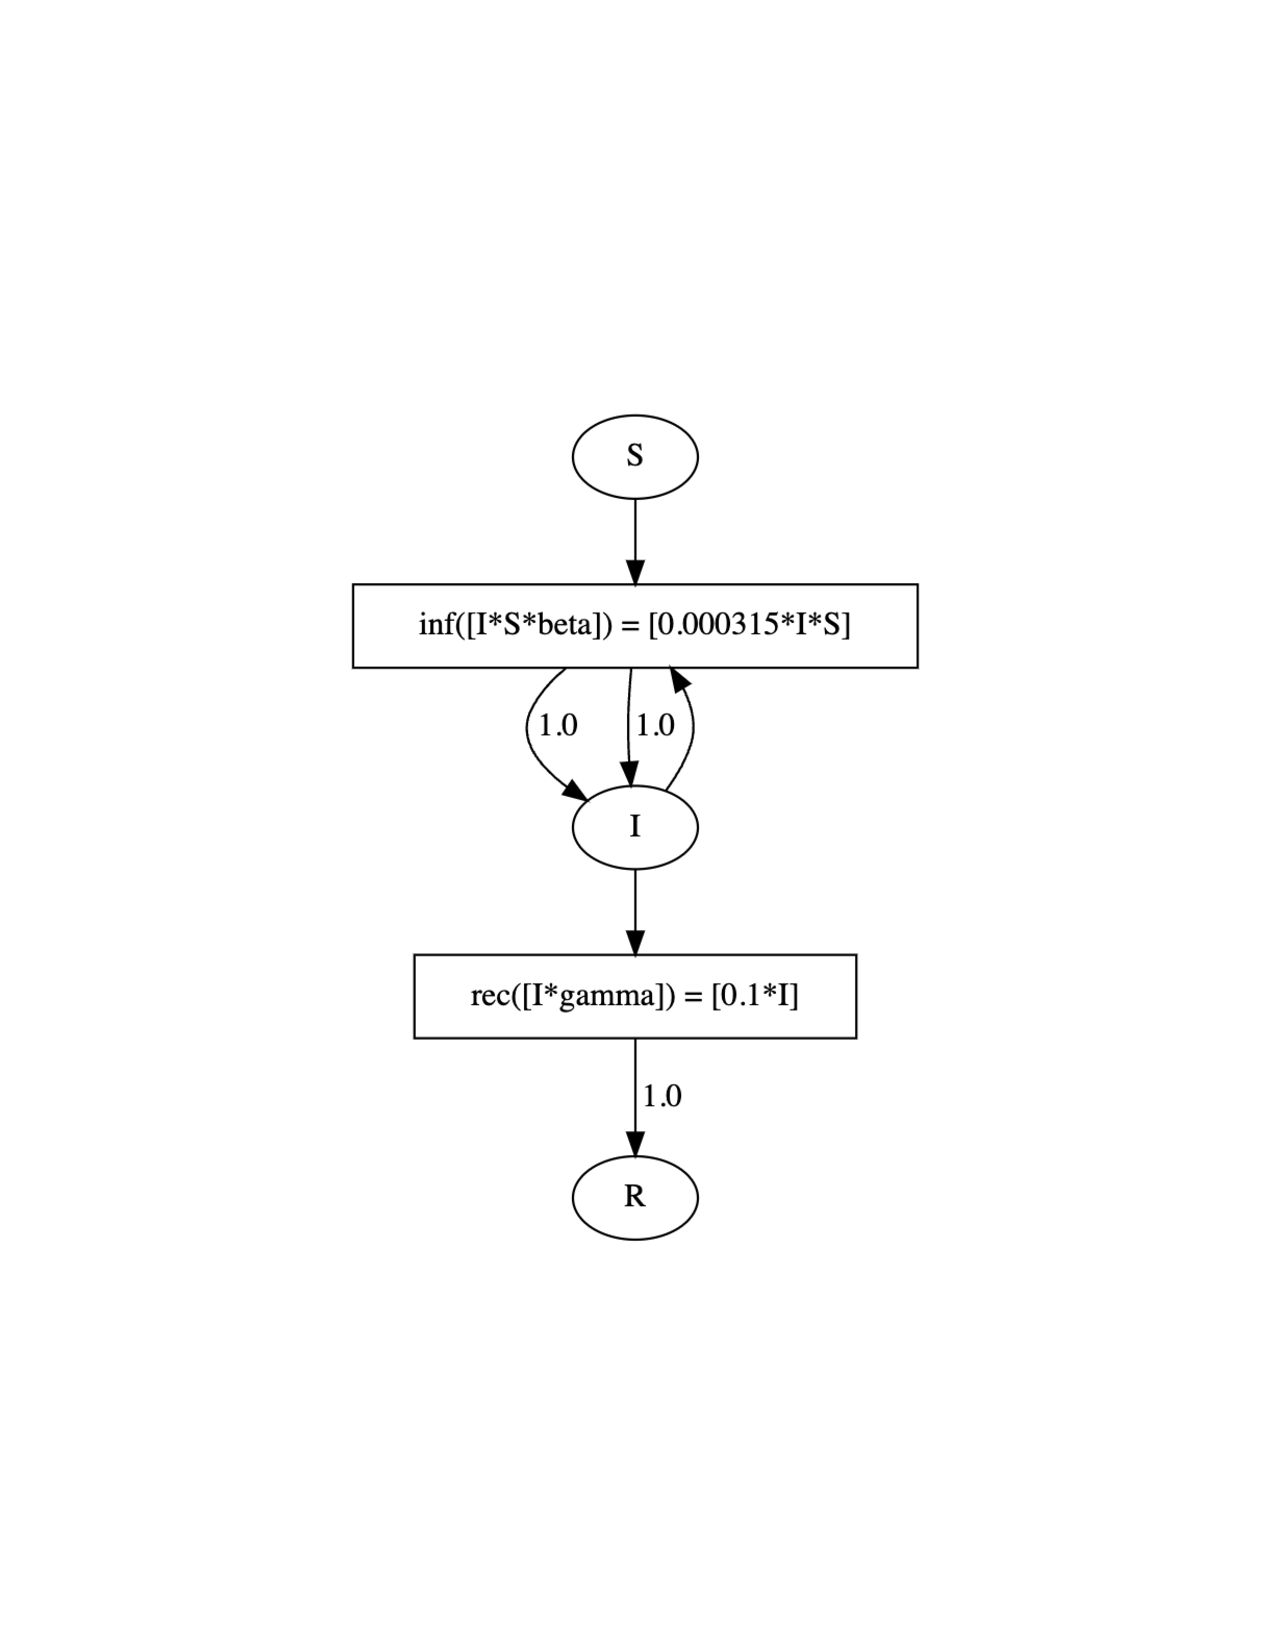
\includegraphics[width=0.3\linewidth,clip]{fig/sir/sir_model.pdf}
    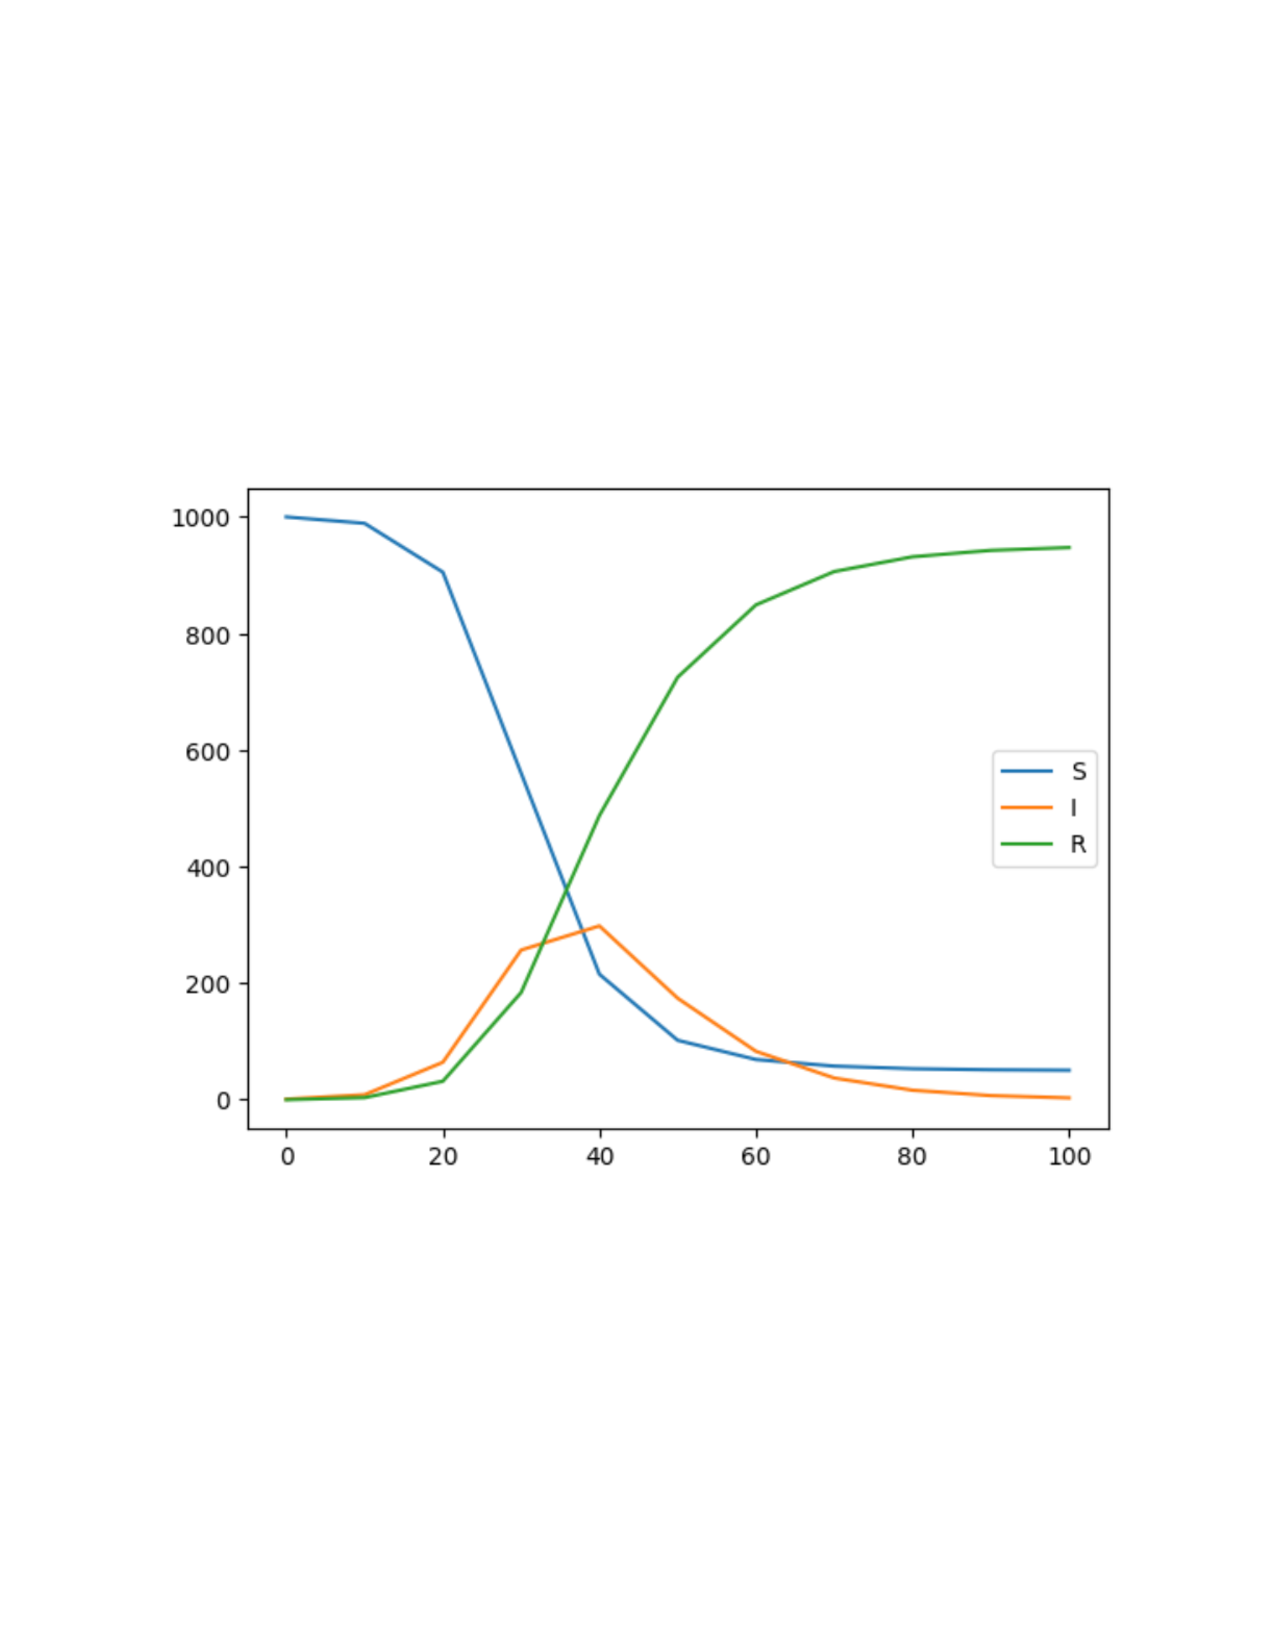
\includegraphics[width=0.4\linewidth,clip]{fig/sir/sir_sim.pdf}

    \caption{\label{fig:sir} Stratified SIR Model (left) and Simulation (right)}
\end{figure}

Figure \ref{fig:sir_bounded} illustrates the baseline SIR after transforming it to bound $S$, $I$, and $R$.  The corresponding lower and upper bounds for each state variable are denoted by a $\_lb$ or $\_ub$ suffix.  The model is different from the baseline in the following ways: there are six state variables and eight transitions, and the transitions use custom rates.  Each baseline transition is replaced by four transitions.  The four transitions differ in whether they define a lower or upper bound, and whether they define the flow into or out from a transition.  For example, the first transition `inf\_in\_lb' defines the lower bound on the flow from $S\_lb$ into the `inf' transition.  The least flow expression is illustrated in the box for the transition.  Simulating this model with the same initial state and parameters (where the lower and upper bounds are initially equal) results in a simulation where the lower and upper bounds are equal for all variables.  While bounding this model in this fashion is not useful in itself, it illustrates a simple application of the bounding transformation.  The bounded abstraction, described below, is similar except that it uses alternative bounds on the parameters.  

\begin{figure}[t]
    \centering
    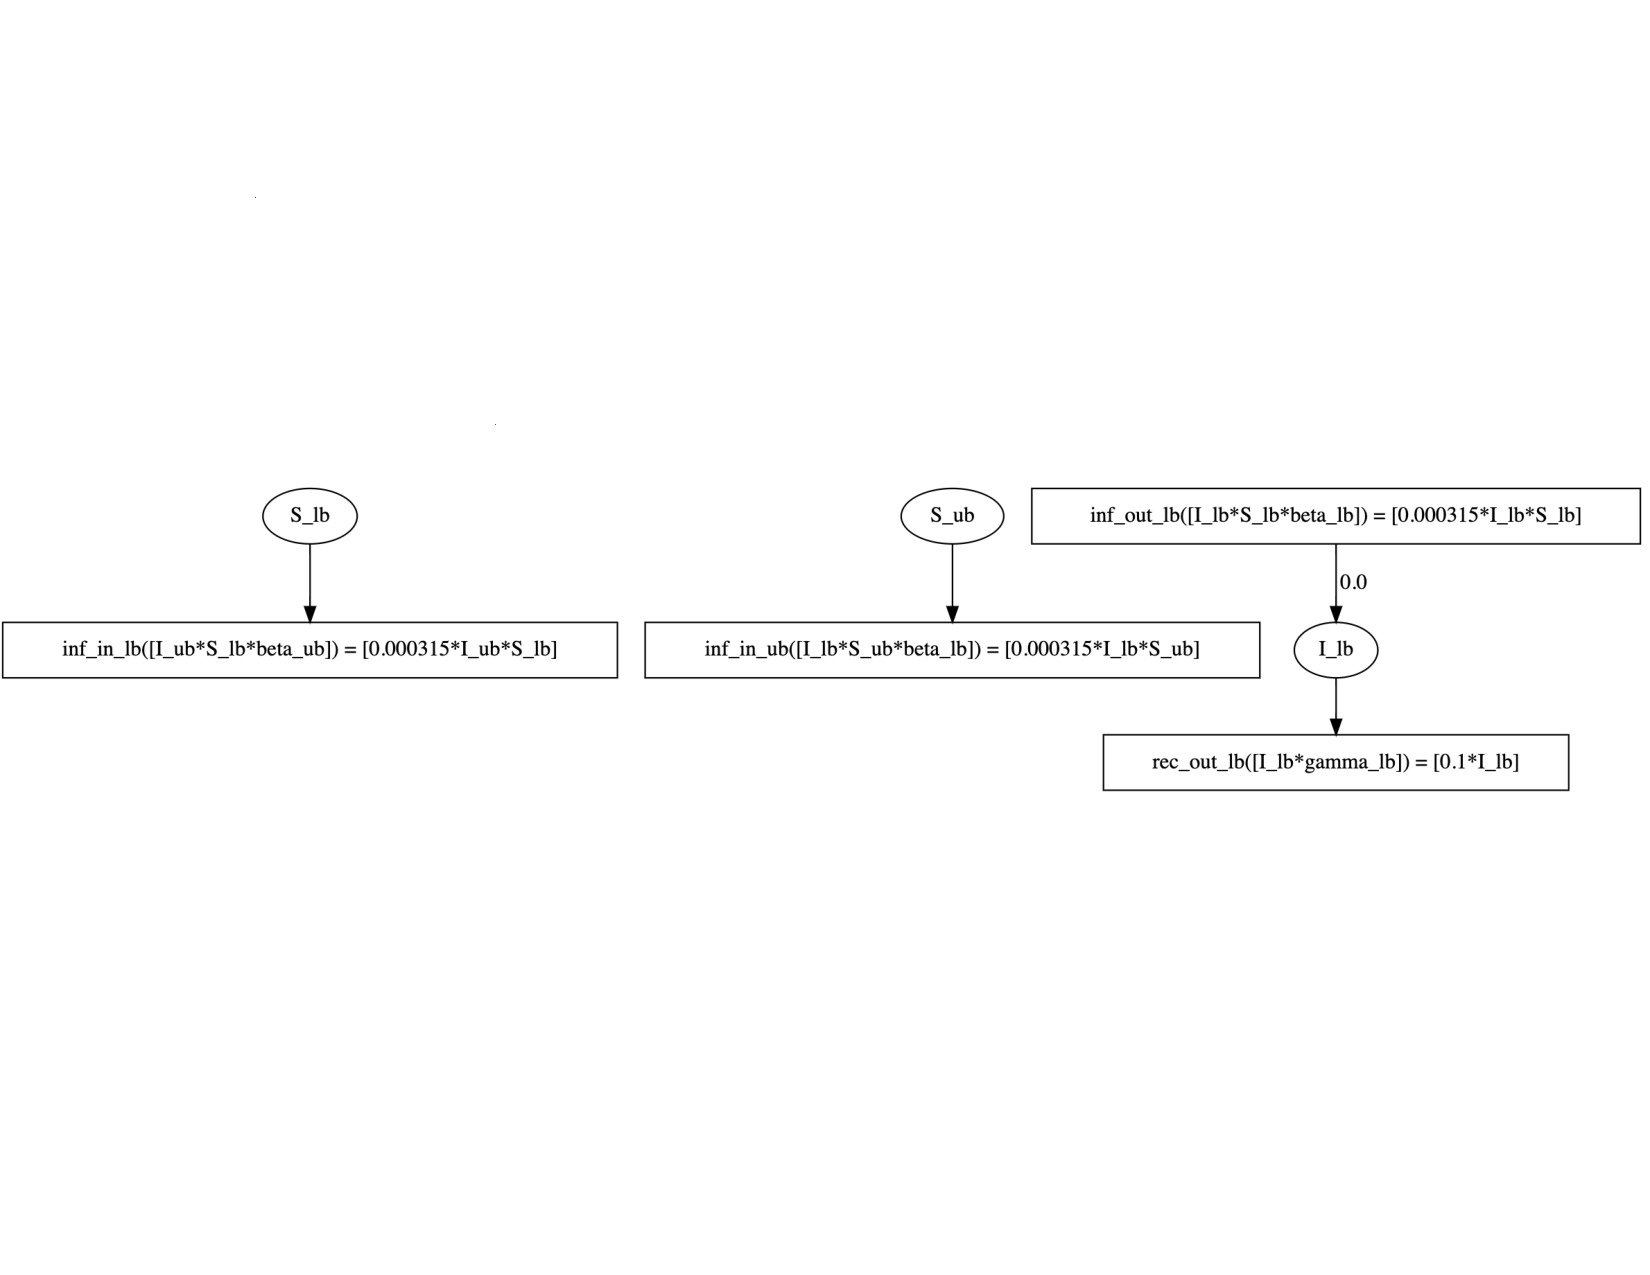
\includegraphics[width=0.8\linewidth,clip,trim={0 8cm 0 8cm}]{fig/sir/sir_bounded_model_1.pdf}
    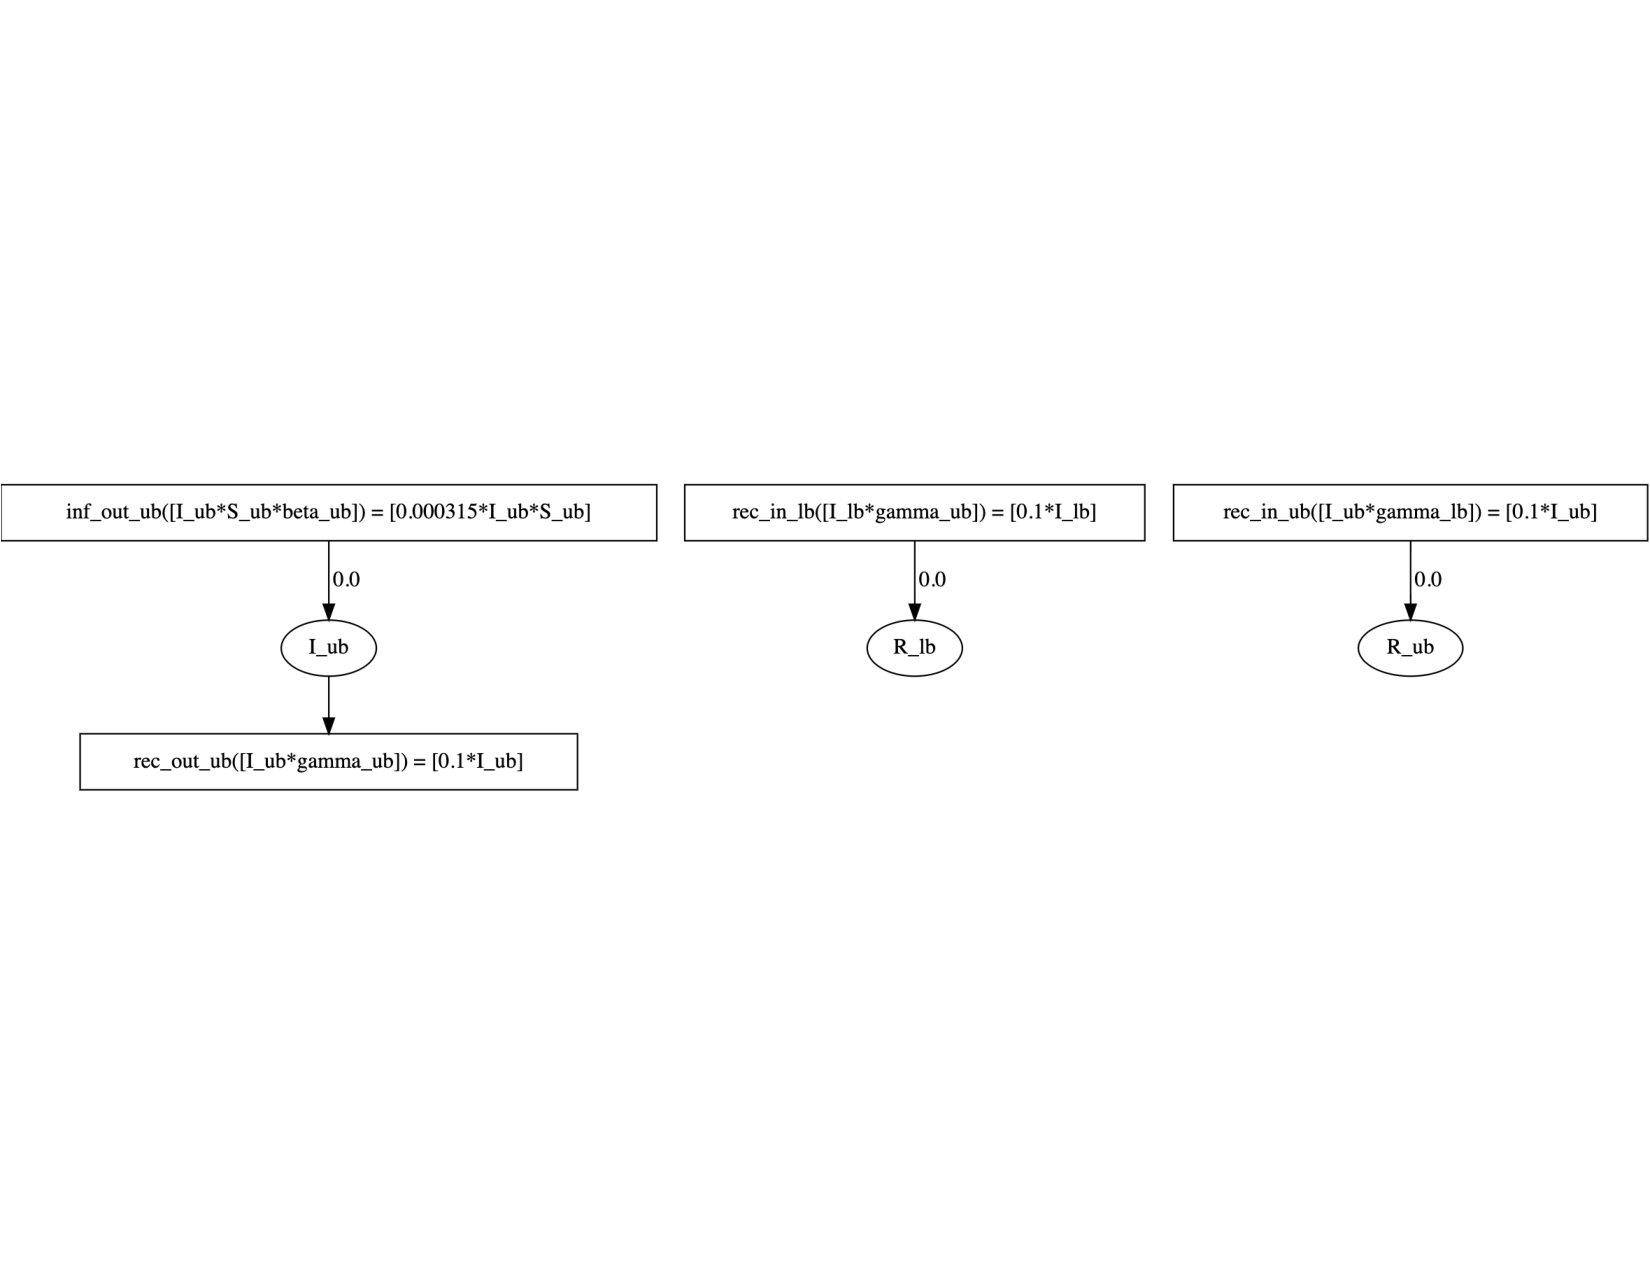
\includegraphics[width=0.8\linewidth,clip]{fig/sir/sir_bounded_model_2.pdf}
    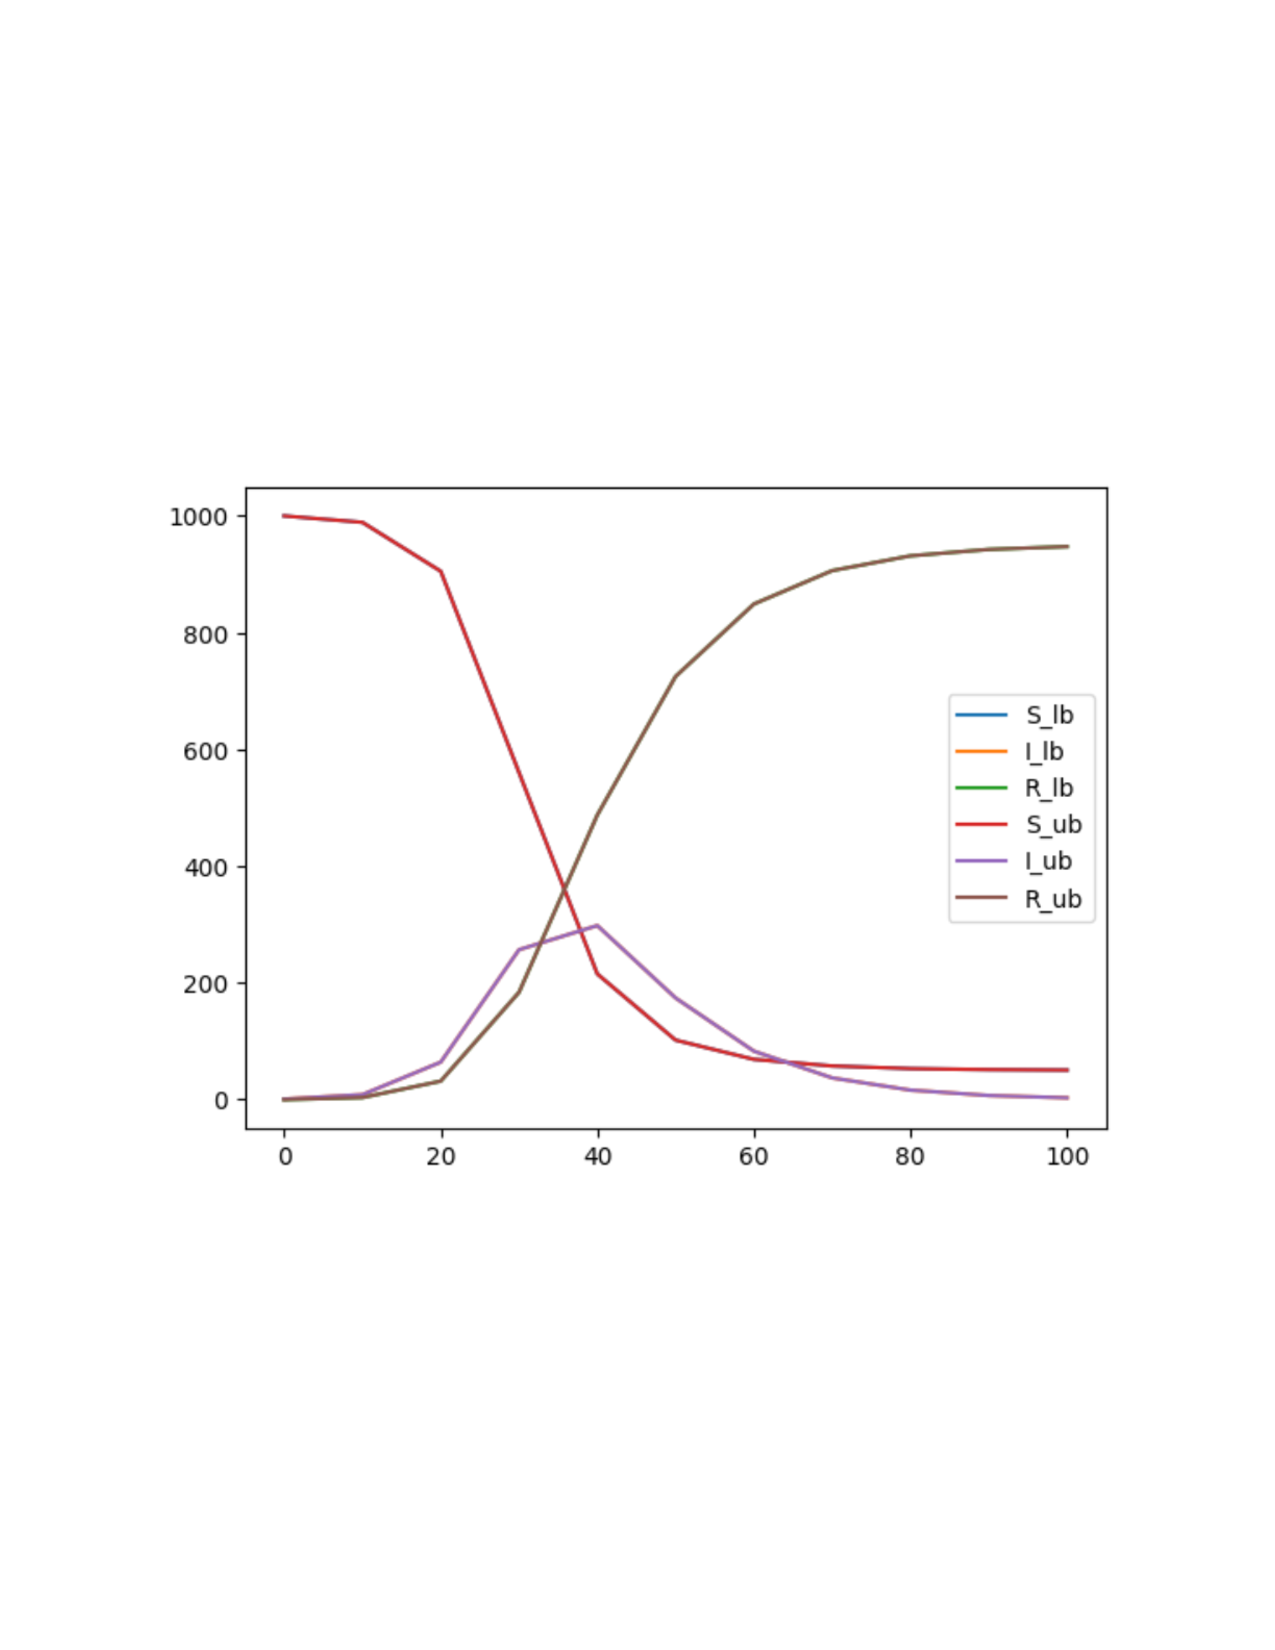
\includegraphics[width=0.4\textwidth,clip]{fig/sir/sir_bounded_sim.pdf}
    \caption{\label{fig:sir_bounded} Bounded SIR Model (top) and Simulation (bottom)}
\end{figure}

Figure \ref{fig:sir_stratified} illustrates the stratified SIR model (wrt. $S$).  It uses state variables that distinguish two $S$ populations and two $inf$ transitions that distinguish different rates due to two $\beta$ parameters.  We modified the $\beta$ parameters to be slightly less and greater than $\beta$ from the previous models.  The simulation illustrates a difference between the $S$ variables.

\begin{figure}[t]
    \centering
    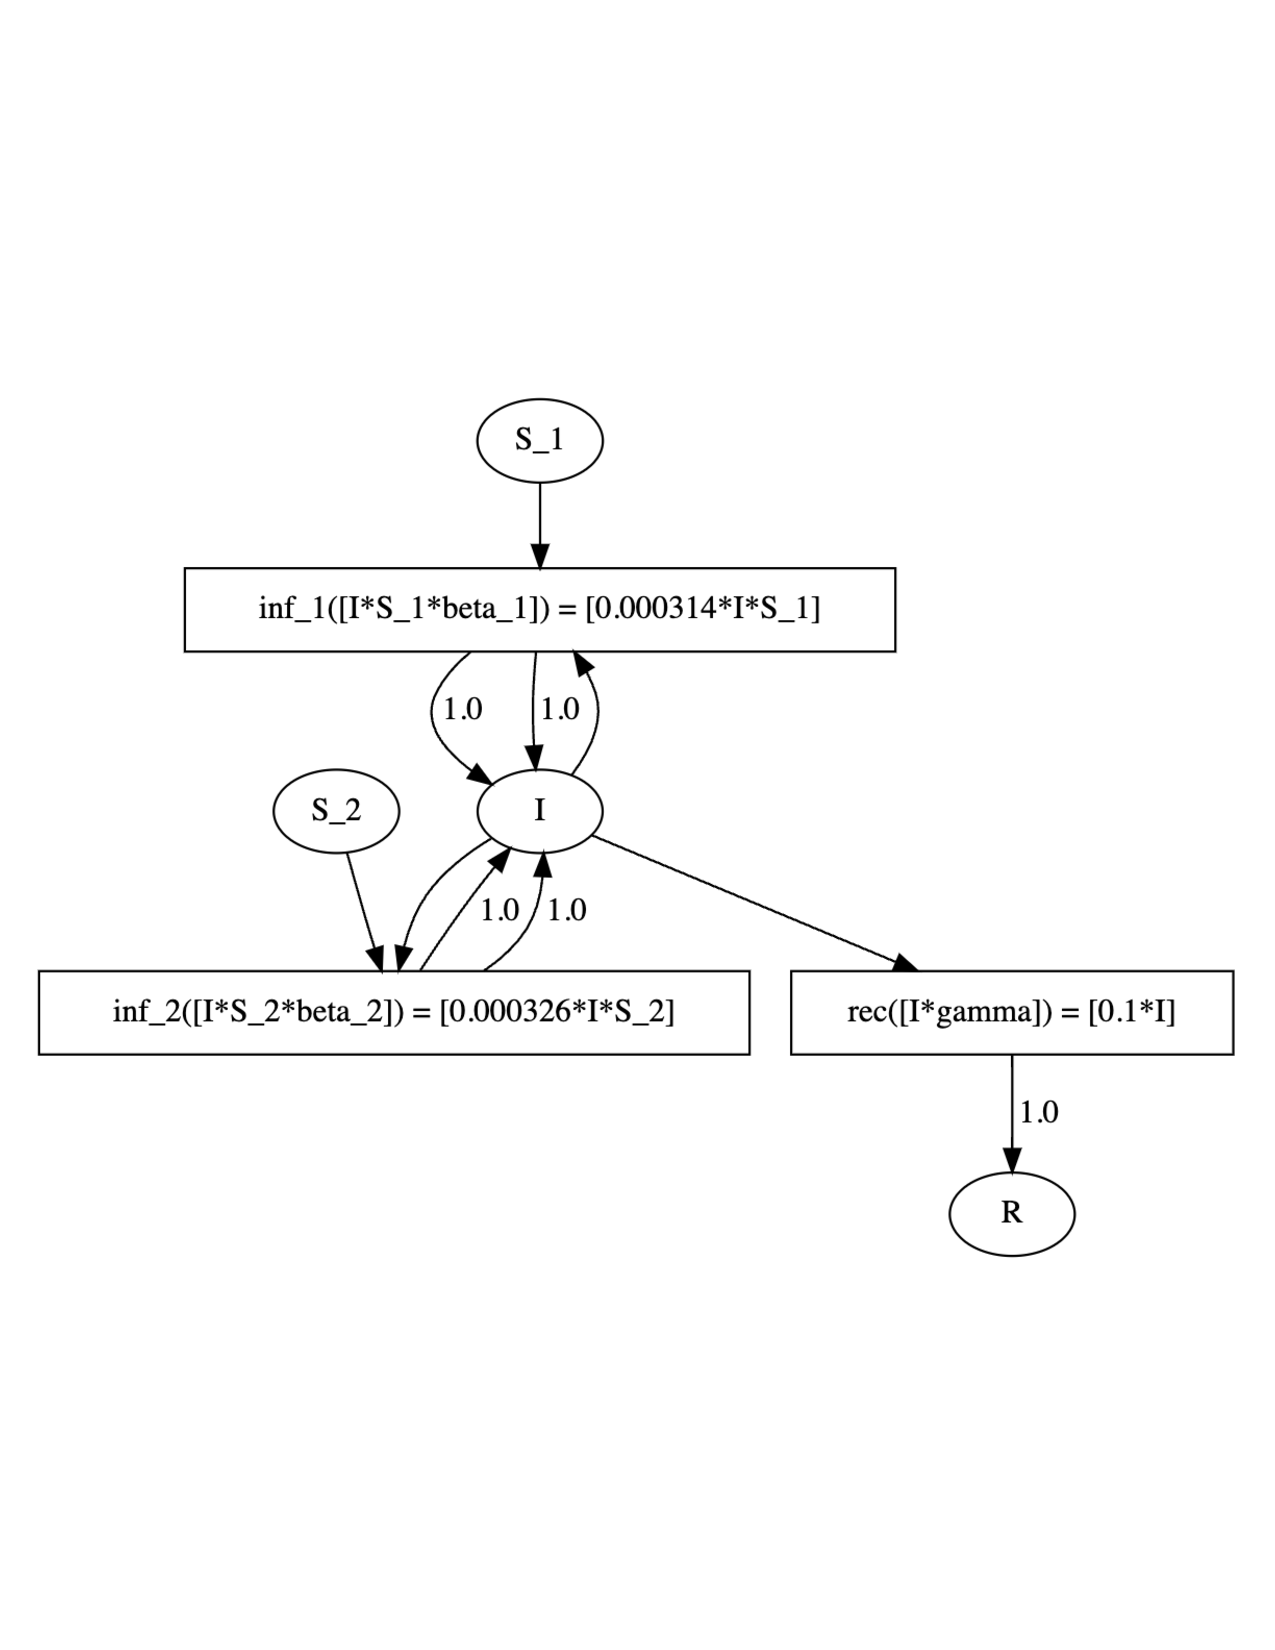
\includegraphics[width=0.5\linewidth,clip]{fig/sir/sir_stratified_model.pdf}
    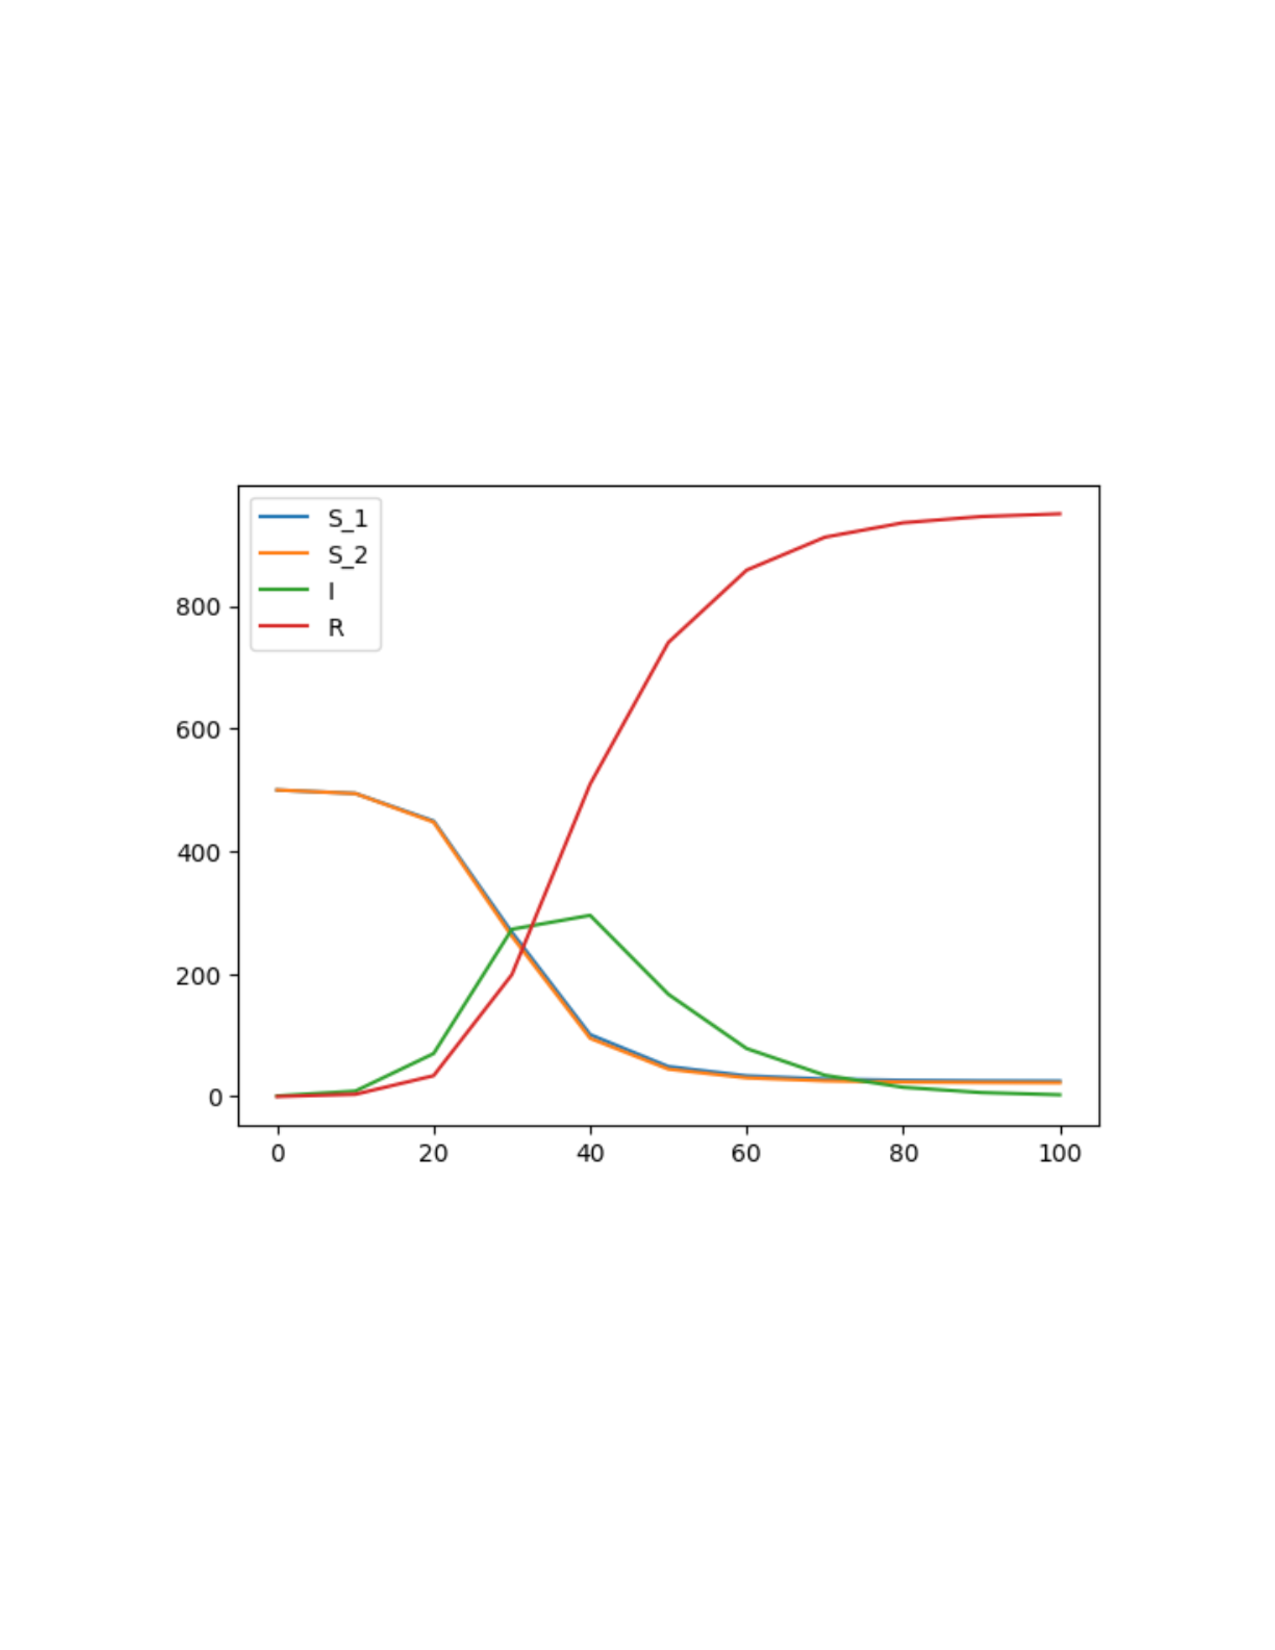
\includegraphics[width=0.4\linewidth,clip]{fig/sir/sir_stratified_sim.pdf}
    \caption{\label{fig:sir_stratified} Stratified SIR Model (top) and Simulation (bottom)}
\end{figure}

Figure \ref{fig:sir_bounded_stratified} illustrates a bounded stratified model, for the sake of illustration.  It resembles the bounded baseline model aside from incorporating the stratified $S$ variable.  The simulation shows how it is possible to bound the stratified variables and achieve similar results to prior models. The primary distinction with this model is how it bounds the stratified variables individually instead of collectively.  The collective bounding can be achieved by first abstracting and then bounding the stratified variables.

\begin{figure}[t]
    \centering
    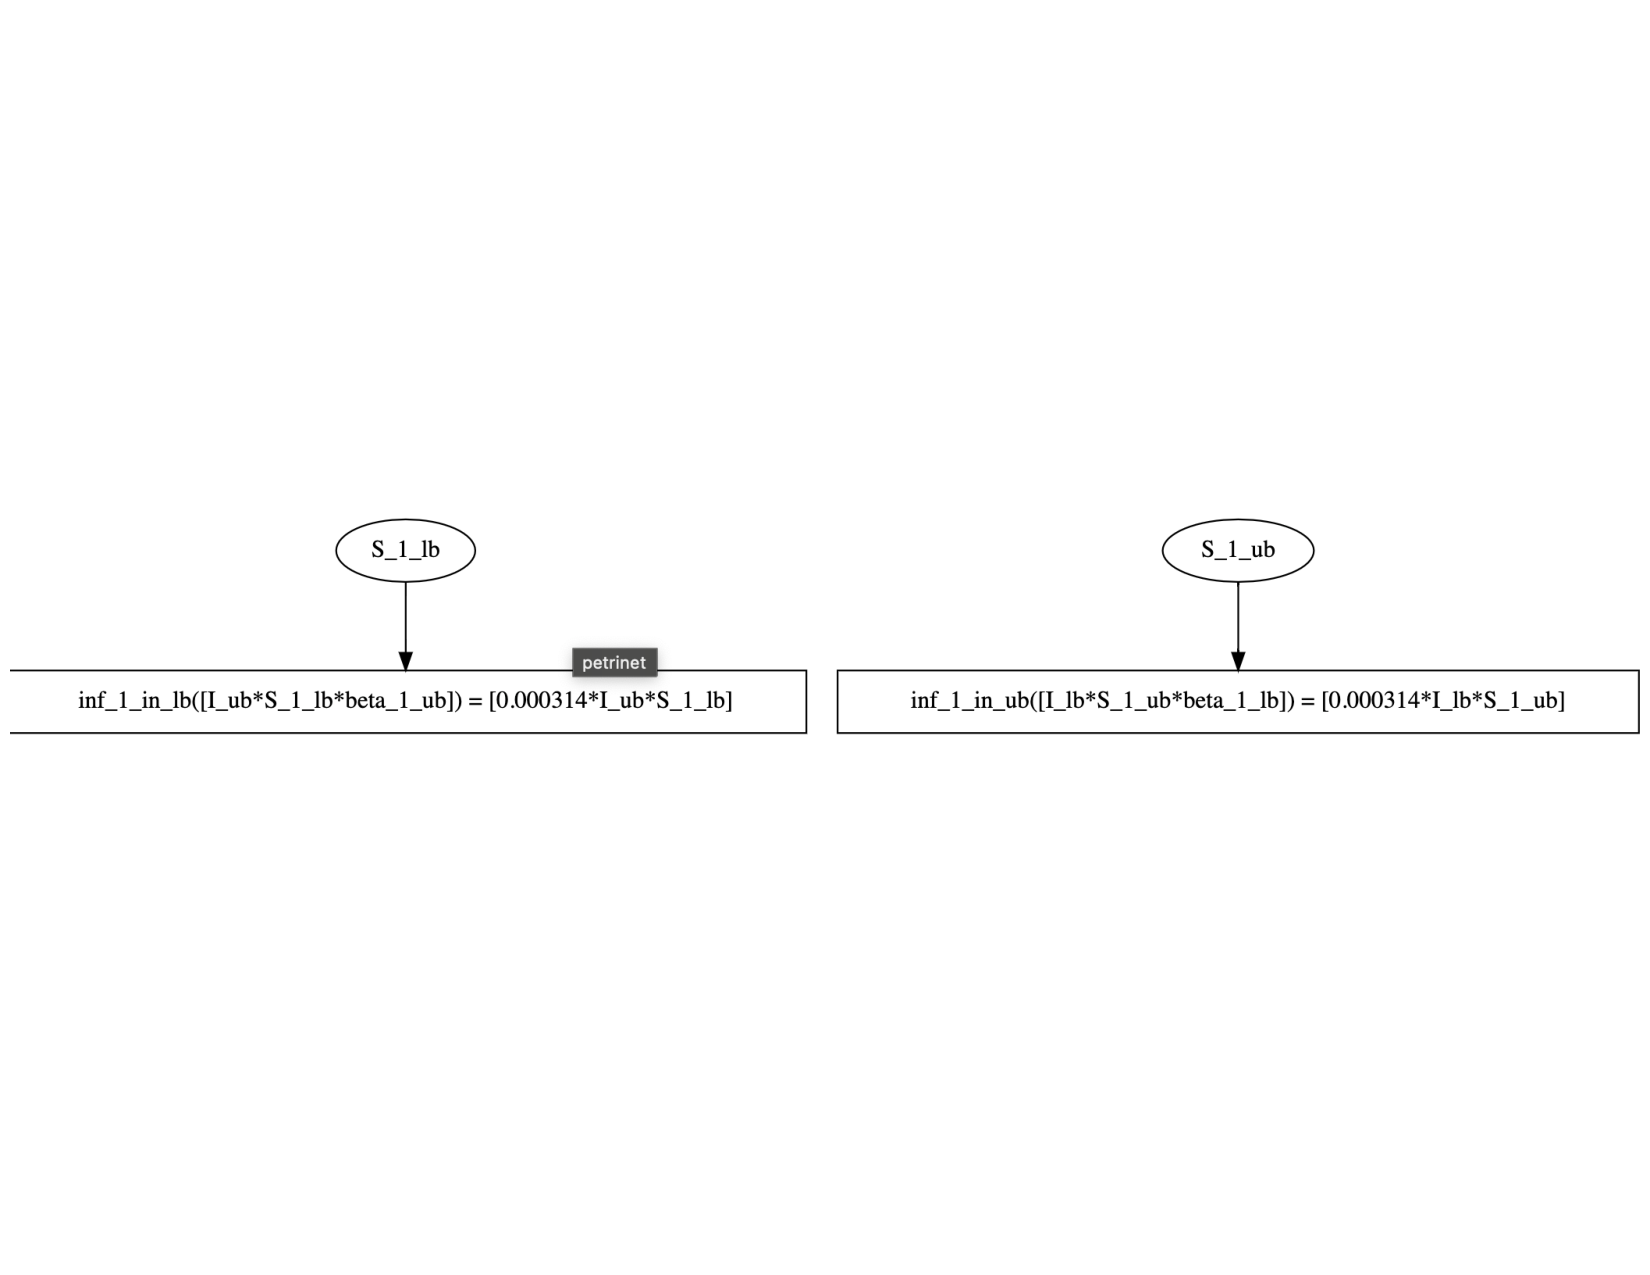
\includegraphics[width=0.6\linewidth,clip]{fig/sir/sir_bounded_stratified_1.pdf}
    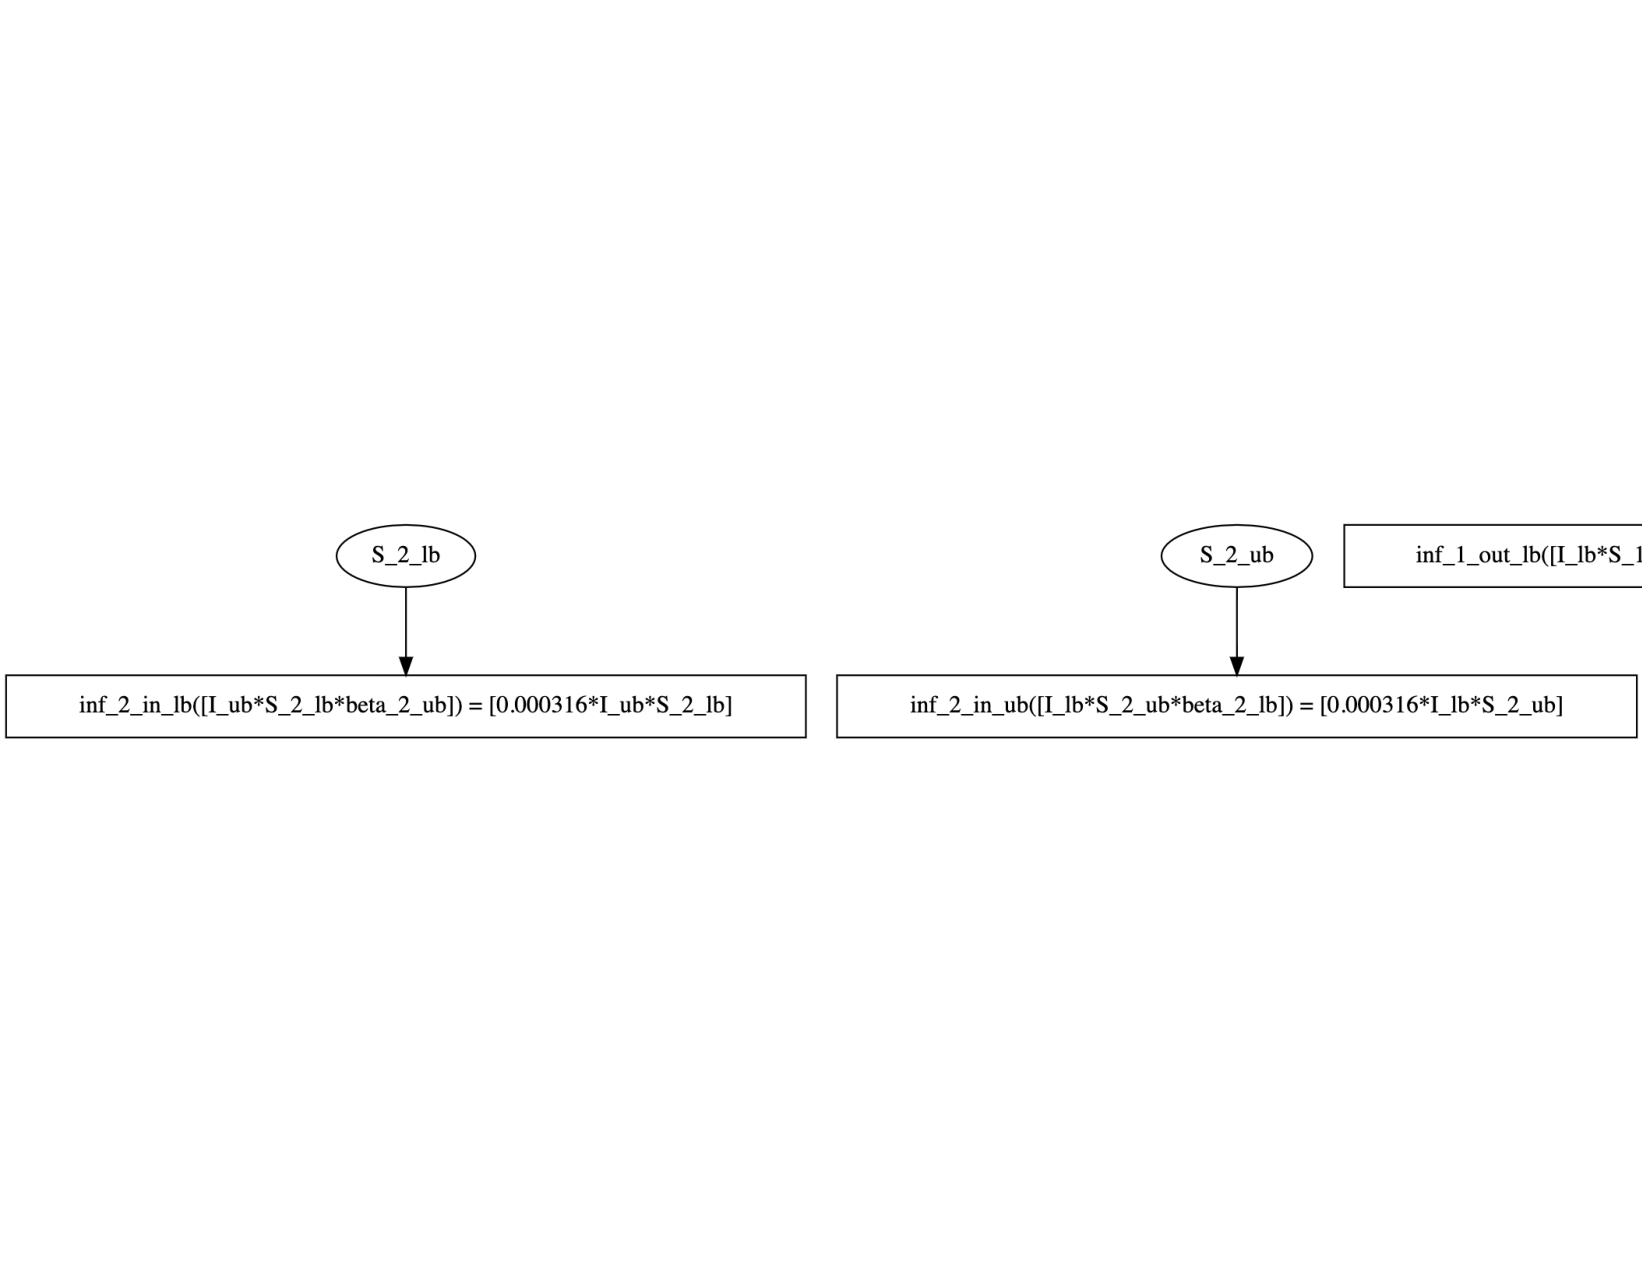
\includegraphics[width=0.6\linewidth,clip]{fig/sir/sir_bounded_stratified_2.pdf}
    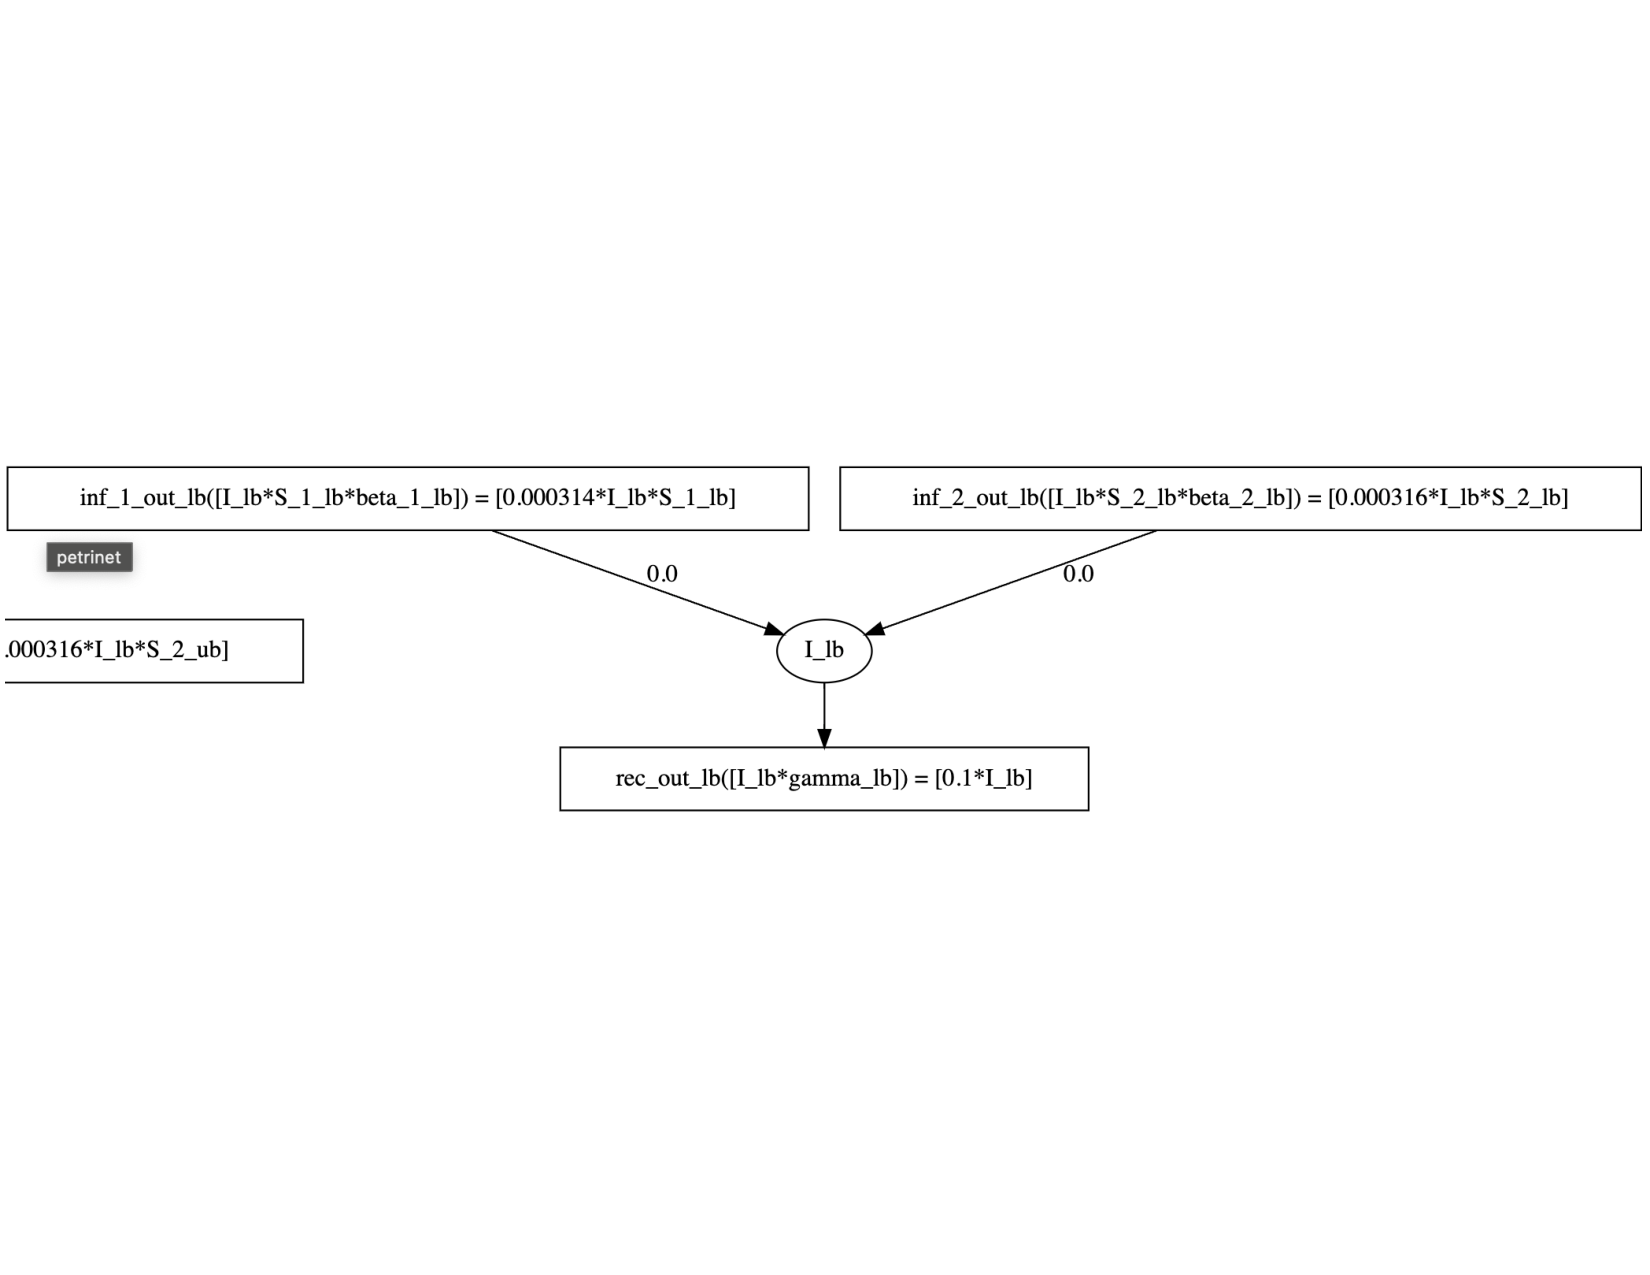
\includegraphics[width=0.6\linewidth,clip]{fig/sir/sir_bounded_stratified_3.pdf}
    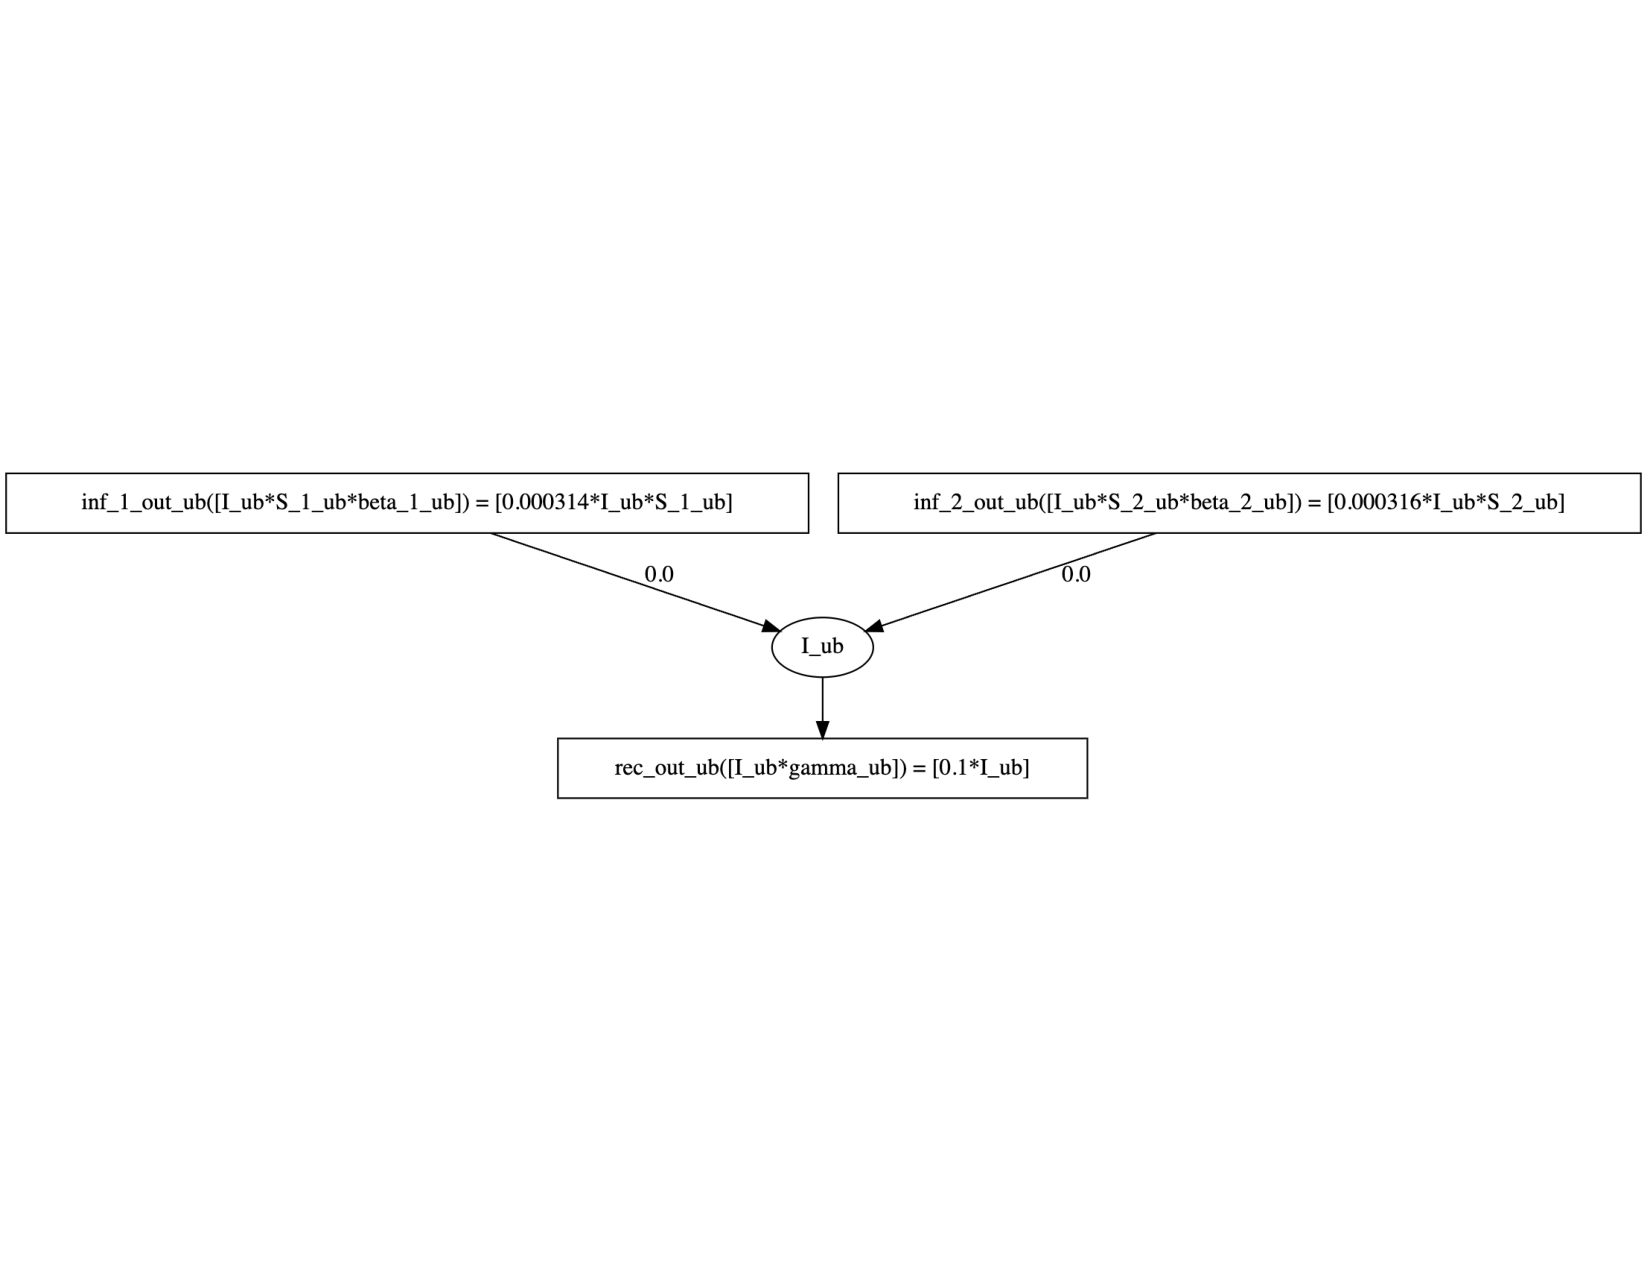
\includegraphics[width=0.6\linewidth,clip]{fig/sir/sir_bounded_stratified_4.pdf}
    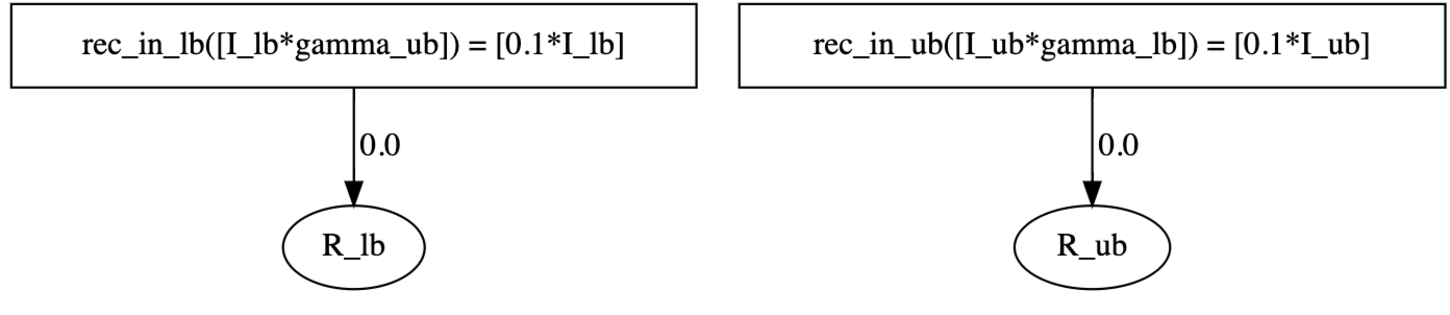
\includegraphics[width=0.4\linewidth,clip]{fig/sir/sir_bounded_stratified_5.pdf}\\
    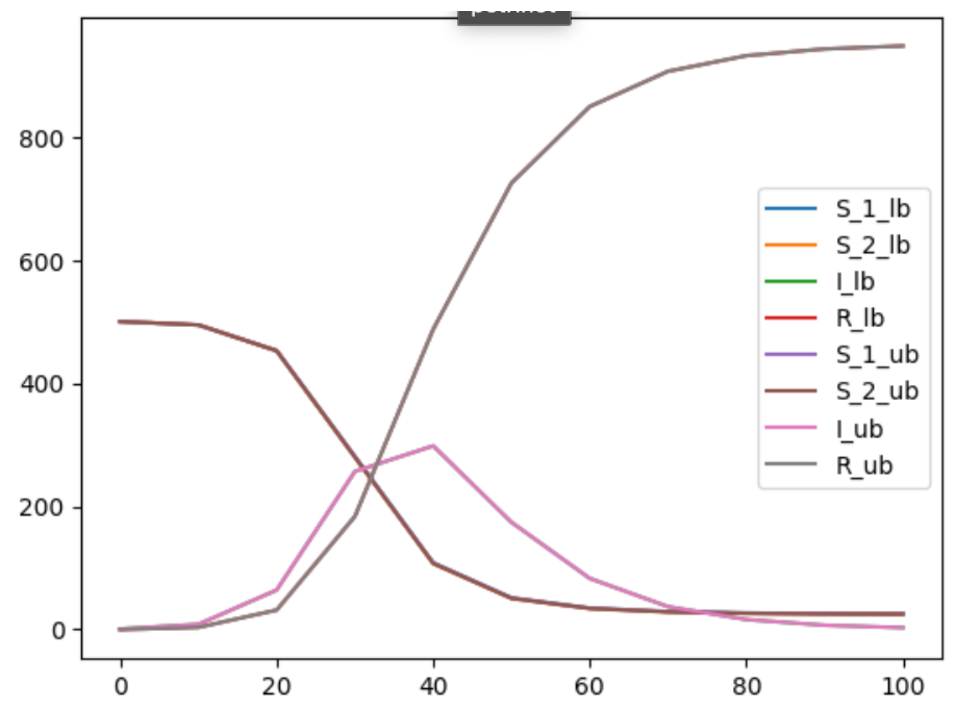
\includegraphics[width=0.4\linewidth,clip]{fig/sir/sir_bounded_stratified_sim.pdf}
    \caption{\label{fig:sir_bounded_stratified} Bounded Stratified SIR Model (top) and Simulation (bottom)}
\end{figure}


Figure \ref{fig:sir_abstract_bounded_stratified}  illustrates the bounded abstracted model.  It resembles the bounded baseline model, except that it incorporates upper and lower bounds on the $\beta$ parameter due to the stratified populations.  By propagating lower and upper bounds that are not equal, this variation of the model captures lower and upper bounds on the abstracted state variables.  The bounds are tight enough to answer several queries about the model.  For example, it can assess whether a upper threshold (that does not fall between the bounds) on peak infected $I$ is satisfied.  The threshold $I \leq 400$ is satisfied because $I\_ub \leq 400$.  However, the threshold $I \leq 300$ may or may not be satisfied because $I\_lb \leq 300 \leq I\_ub$.

\begin{figure}[t]
    \centering
    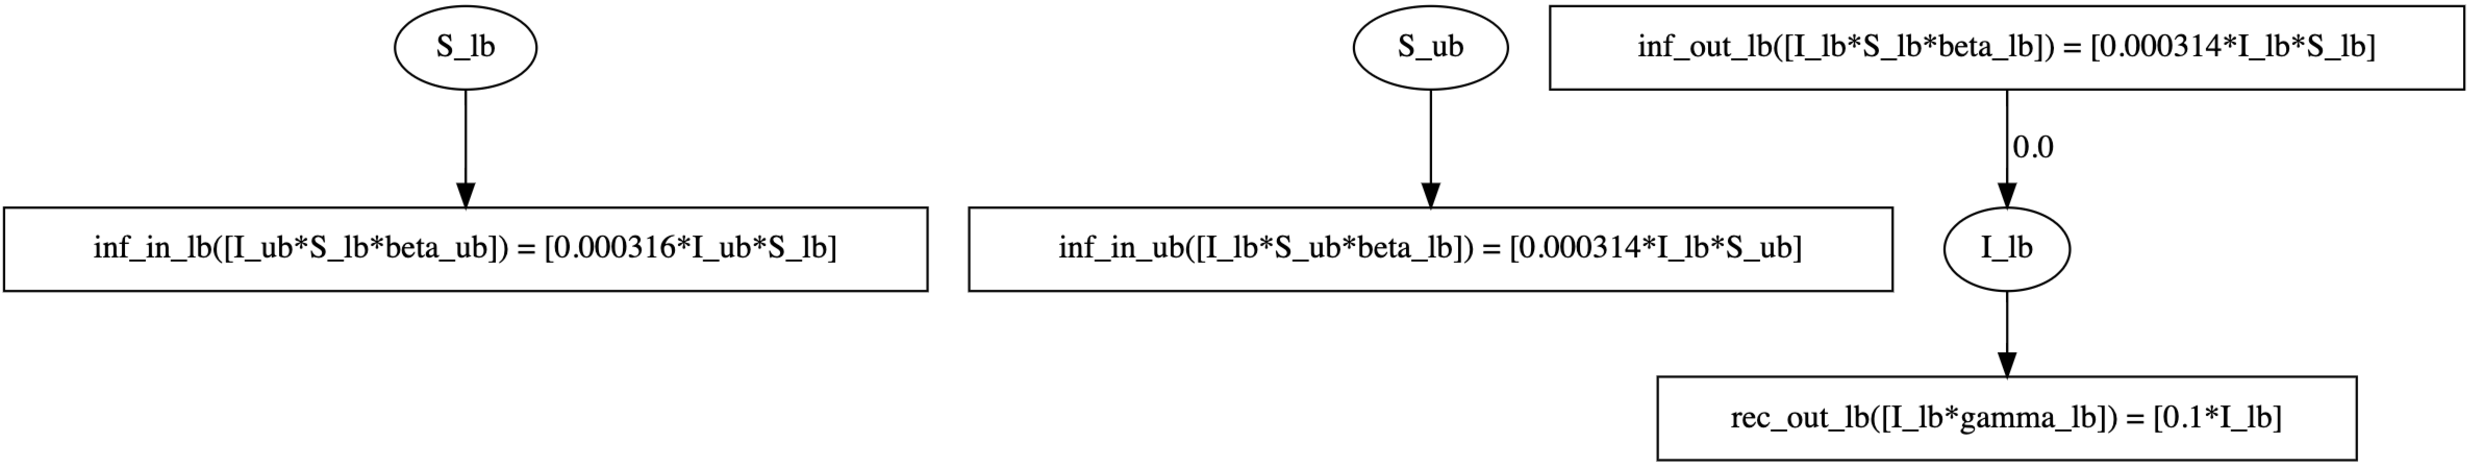
\includegraphics[width=0.6\linewidth,clip]{fig/sir/sir_abstract_bounded_model_1.pdf}
    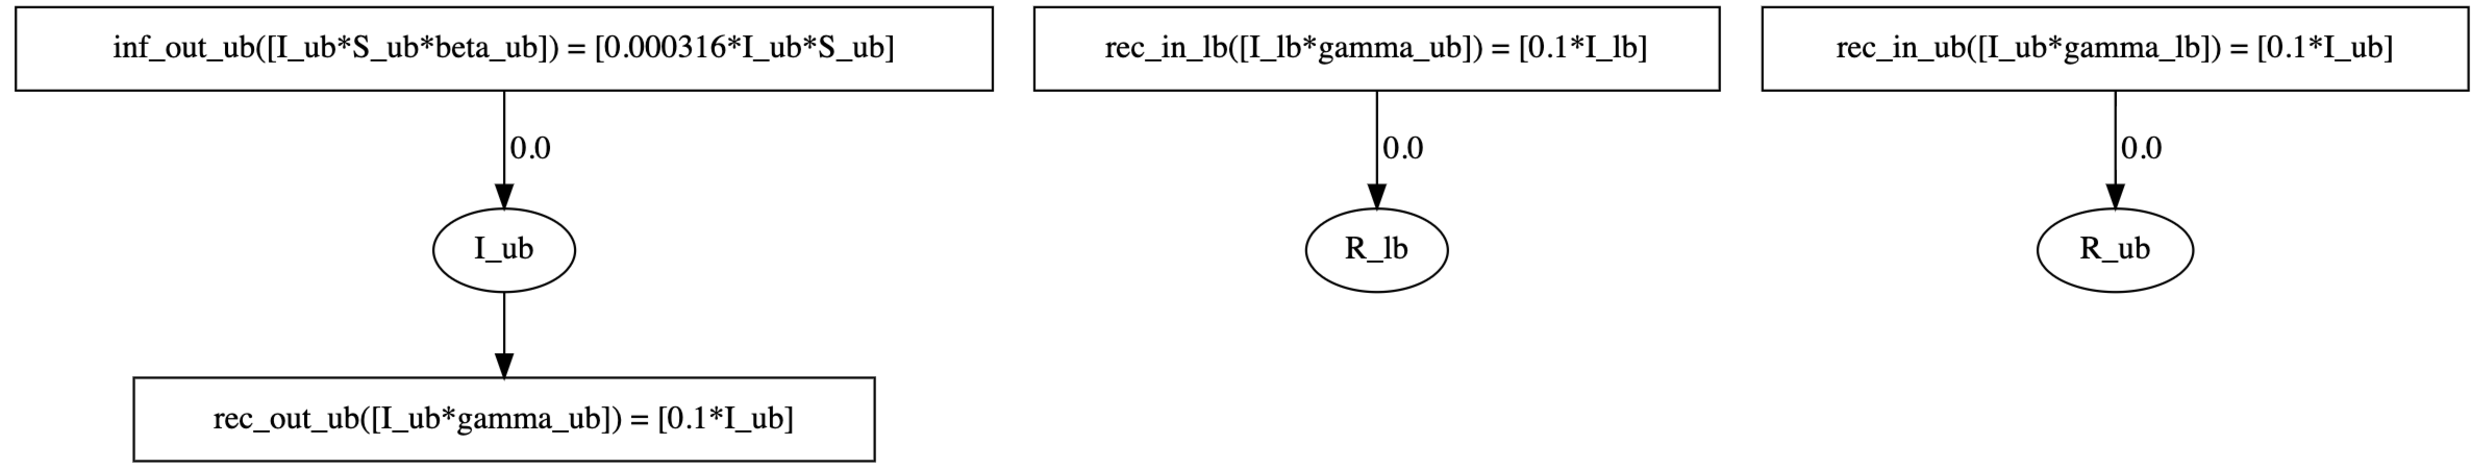
\includegraphics[width=0.6\linewidth,clip]{fig/sir/sir_abstract_bounded_model_2.pdf}
    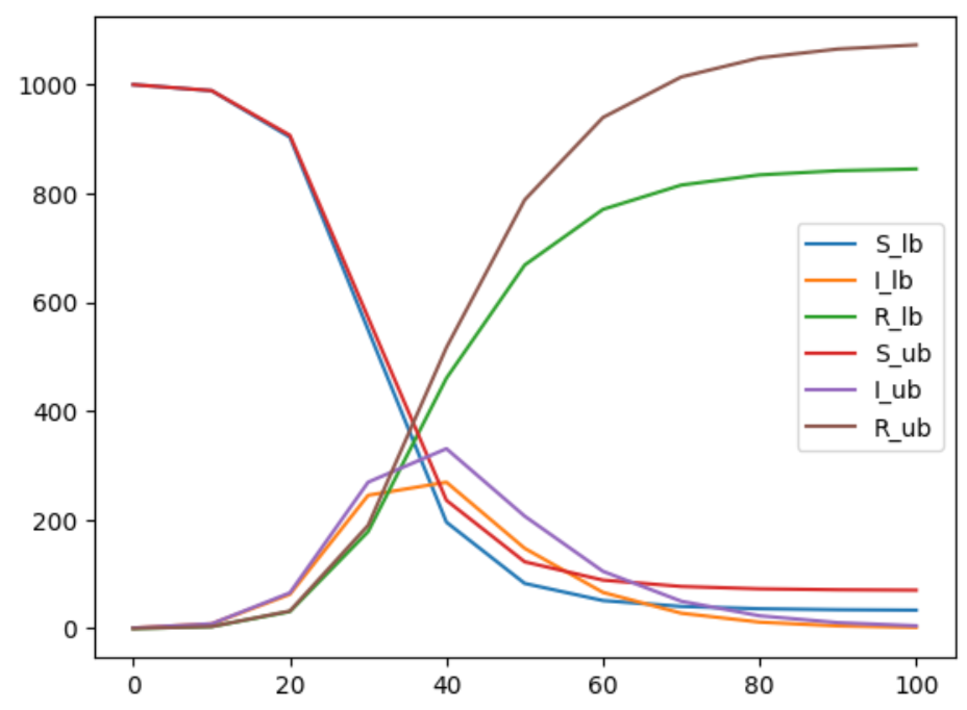
\includegraphics[width=0.4\linewidth,clip]{fig/sir/sir_abstract_bounded_sim.pdf}
    \caption{\label{fig:sir_abstract_bounded_stratified} Bounded Stratified SIR Model (top) and Simulation (bottom)}
\end{figure}

% \begin{figure}
%     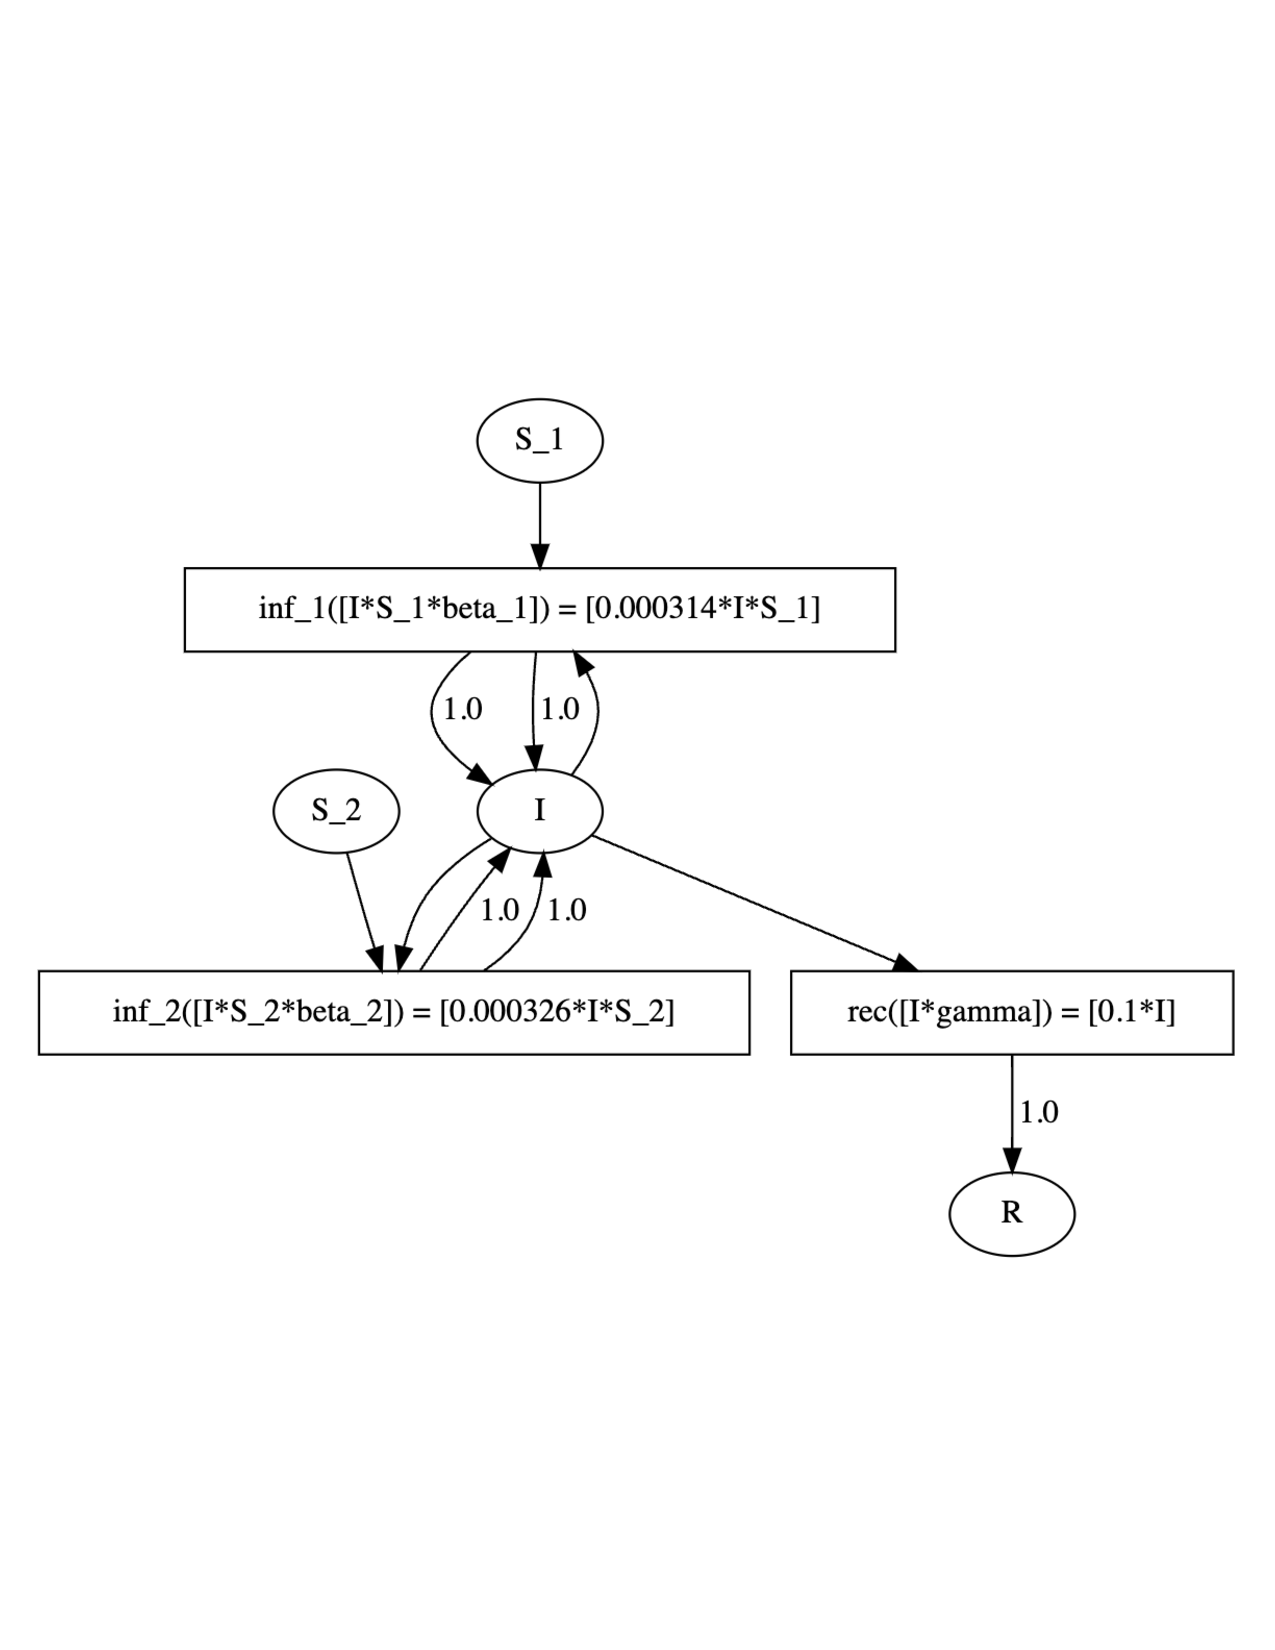
\includegraphics[width=\linewidth]{fig/sir/sir_stratified_model.pdf}
% %     \caption{\label{fig:sir_stratified_model} Stratified SIR Model}
% % \end{figure}

% % \begin{figure}
%     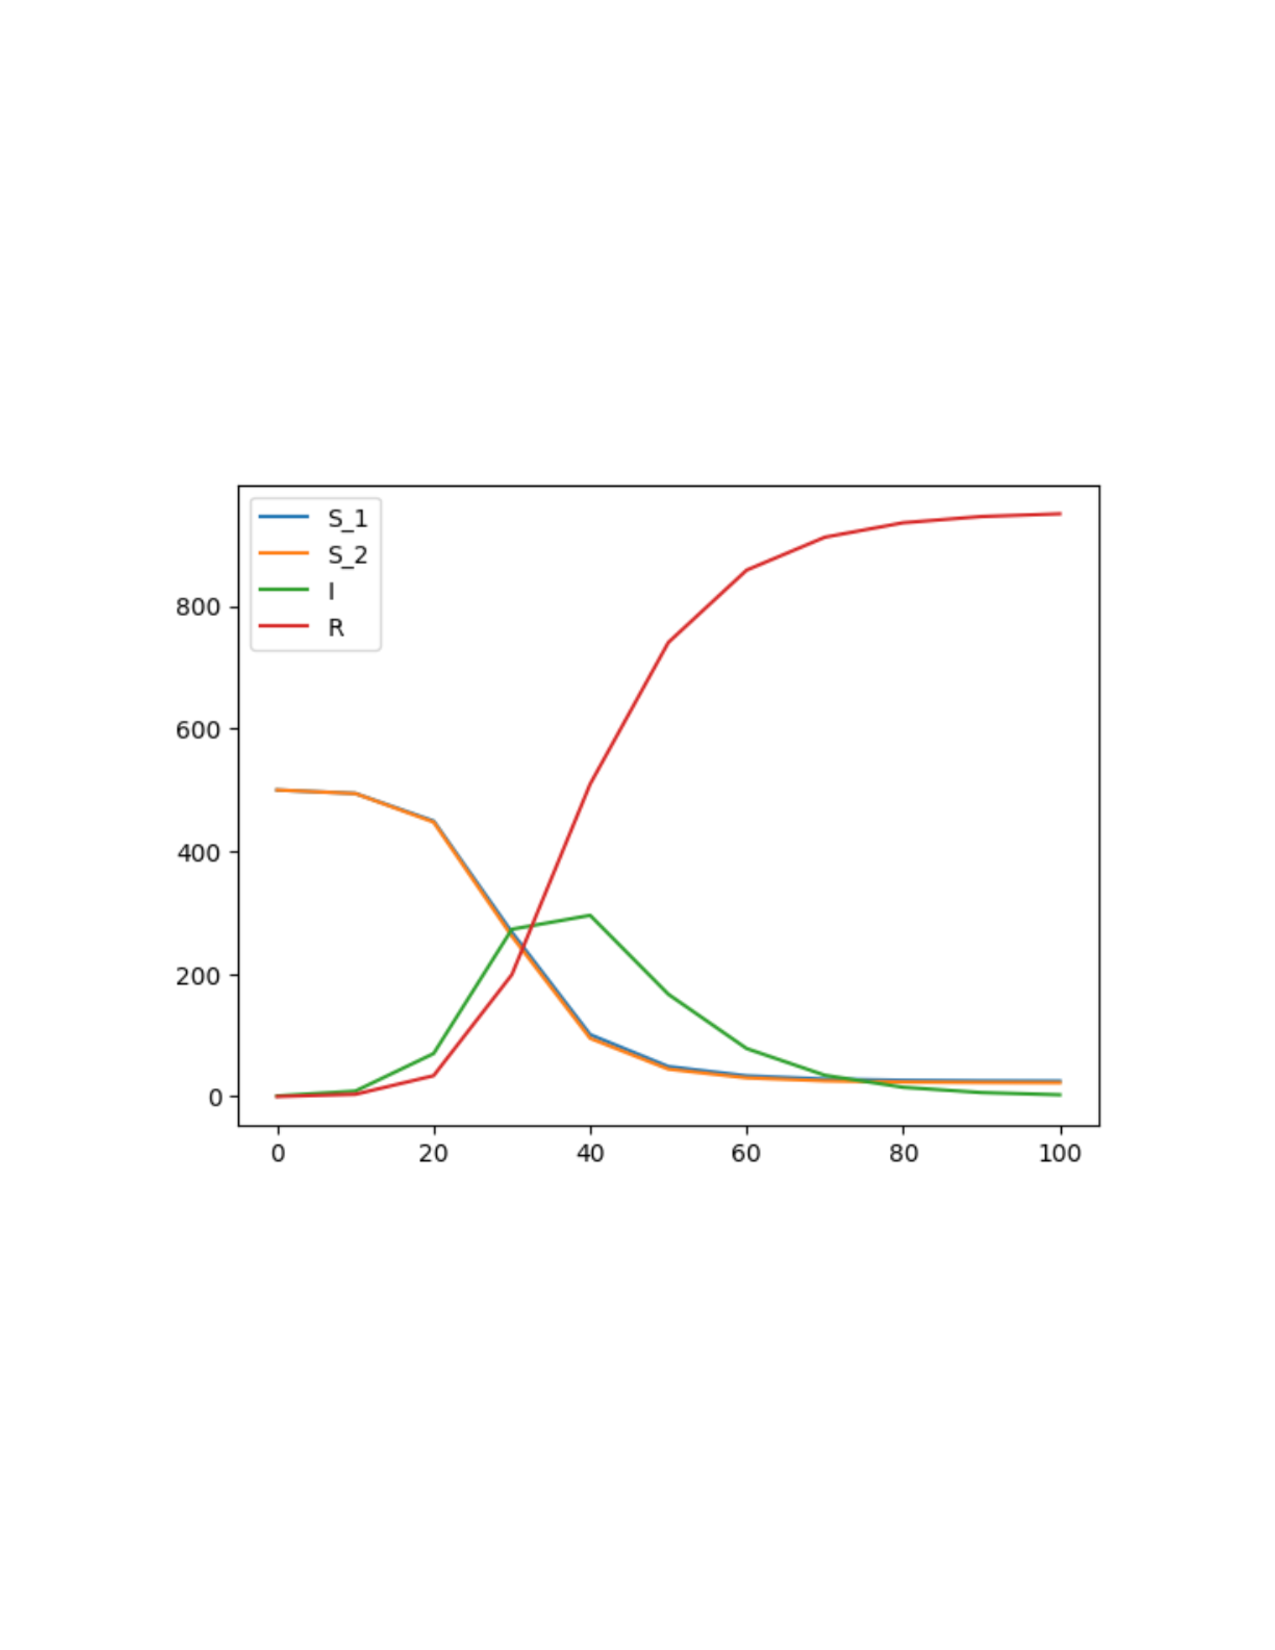
\includegraphics[width=\linewidth]{fig/sir/sir_stratified_sim.pdf}
%     \caption{\label{fig:sir_stratified_sim} Stratified SIR Model (top) and Simulation (bottom)}
% \end{figure}